%!TEX root = main.tex
\clearpage
\section{Conclusion}

\subsection{Global Vision}

In table \ref{tab:operators_status}, it's possible to understand the operators that were implemented in the first semester of this dissertation. As can be seen, I have implemented \red{five} of thirteen operators that João Durães specified.

In table \ref{tab:constraints_status}, is also possible to check that I have implemented \red{three} of eleven constraints related to the thirteen operators.

% \clearpage
\begin{table}[ht]
\begin{tabular}{c}
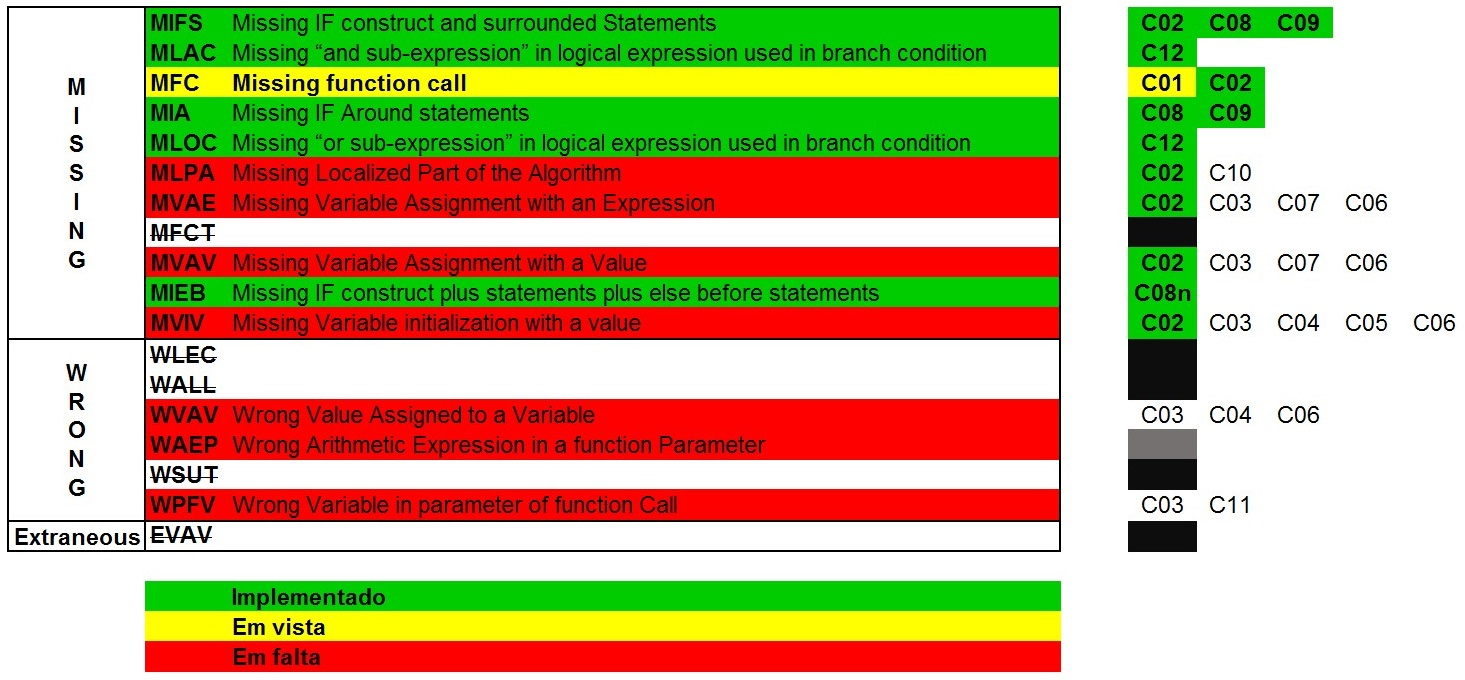
\includegraphics[width=1.1\textwidth]{img/operators_status.jpg}
\end{tabular}
\caption{\small \sl State of the operators and its constraints.\label{tab:operators_status}}
\end{table}



\begin{table}[ht]
\begin{tabular}{c}
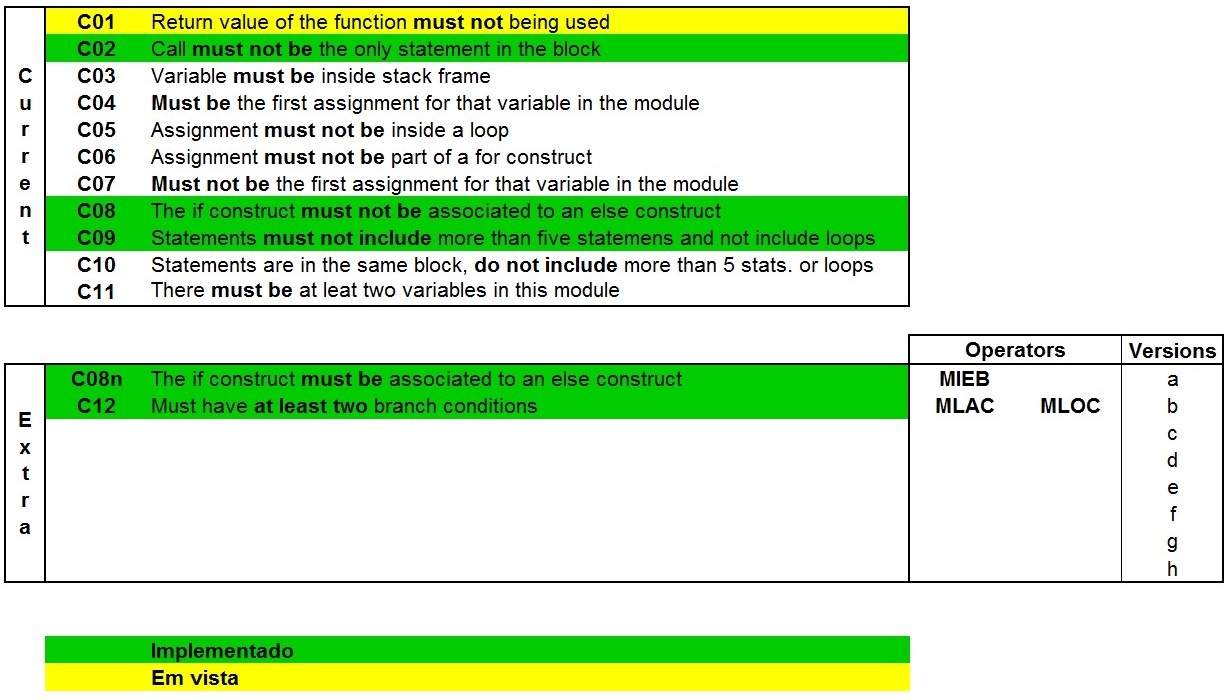
\includegraphics[width=1.1\textwidth]{img/constraints_status.jpg}
\end{tabular}
\caption{\small \sl State of the constraints.\label{tab:constraints_status}}
\end{table}

\clearpage
\subsection{Future Work}

\iftoggle{long}{\orange{Mais do que “future work” é necessário um plano para o segundo semestre, relativamente detalhado.}}

\iftoggle{long}{\orange{Globalmente há várias coisas que não estão suficientemente bem explicadas:}}

\iftoggle{long}{\orange{- exatamente quais são as características novas da cloud, que devem ser avaliadas por injeção de falhas (podemos conversar sobre isto)}}

\iftoggle{long}{\orange{- qual a razão para se desenvolver algo novo, quando a ferramenta do Natella já faz muito (lembro-me que colecionámos muitos argumentos}}

\iftoggle{long}{\orange{que estão anotados)}}

\iftoggle{long}{\orange{- como é que se vai dar uso ao que está implementado? far-se-ão experiências, os resultados serão classificados e analisados certamente}}

\iftoggle{long}{\orange{- o estado da arte deveria ponderar os prós e os contras de todas as técnicas para injeção de falhas de software (binário, instrumentação, source}}

\iftoggle{long}{\orange{code, runtime, etc.)}}

\iftoggle{long}{\orange{- o texto deve ser clarificado, mas essencialmente é no plano das ideias que muitas vezes está pouco claro: por que razão se está a fazer isto?}}

\iftoggle{long}{\orange{quais são as alternativas? como é feito? exatamente o que é feito}}

In the future, I have planned to implement the other operators and constraints. In addition, apply this software in testing of open source software's that I will select.

I will use \red{regression testing} to verify if when I coded one new operator or constraint I didn't mess with the operators and constraints previous implemented.
\red{From version to version, I use a regression testing to test the fault injector to guarantee that application doesn't regarded.}


\textit{``The purpose of regression testing is to ensure that changes made to software, such as adding new features or modifying existing features, have not adversely affected features of the software that should not change. Regression testing is usually performed by running some, or all, of the test cases created to test modifications in previous versions of the software.''}

\iftoggle{long}{\red{Regression Testing}}


\iftoggle{long}{\red{System testing}}


\iftoggle{long}{\red{Unit tests}}

% \clearpage
% \subsubsection{Applications to inject faults}

\iftoggle{long}{
	\hypertarget{Applications_to_inject_faults}{}
 	\subsubsection{Applications to inject faults}
 	\bookmark[level=\thesubsubsection,dest=Applications_to_inject_faults]{\thesubsubsection \ Applications to inject faults}
}

% \red{The same applications that João Durães has collected information?}
% \begin{itemize}
% 	\item MinGW, Last Update: 2015-06-08
% 	\item ScummVM, Last Update: 2015-05-17
% 	\item CDEX, Last Update: 2015-04-24
% 	\item FireBird, Last Update: 2015-04-15
% 	\item Joe, Last Update: 2015-03-22
% 	\item FreeCiv, Last Update: 2015-03-14
% 	\item GAIM or Pidgin, Last Update: 2015-01-07
% 	\item BASH, Last Update: 2013-12-10
% 	\item ZSNES, Last Update: 2013-05-07
% 	\item VIM, Last Update: 2013-04-25
% 	\item pdftohtml, Last Update: 2013-04-24
% 	%\item LKERNEL
% \end{itemize}
